\section{Gradient Descent, MLE and Odds}
\subsection{Gradient Descent}
Gradient descent is an optimization algorithm that finds the best parameters across many tasks, such as linear or logistic regression and neural networks.
\begin{algorithm}
\caption{Gradient Descent Optimization}
\begin{algorithmic}[1]
\Require Learning rate $\alpha > 0$, maximum iterations $max\_iter$, convergence threshold $\epsilon > 0$

\State $\nabla L(\theta) = [\frac{\partial L}{\partial \theta_1}, \frac{\partial L}{\partial \theta_2}, \ldots, \frac{\partial L}{\partial \theta_n}]$ \Comment{$L(\theta)$ loss function, $\theta = [\theta_1, \theta_2, \ldots, \theta_n]$}
\State $\bar\theta=[\bar\theta_1,\bar\theta_2,...,\bar\theta_n]$, with  $\bar\theta_i$ randomly chosen\Comment{parameter initialization}
\State $iter \gets 0$
\State $step\_size \gets \infty$

\While{$step\_size > \epsilon$ \&\& $iter < max\_iter$}
    \State $g \gets \nabla L(\bar\theta)$ \Comment{evaluate gradient}
    \State $step\_size \gets \|g\| \times \alpha$ \Comment{calculate stepsize}
    \State $\bar\theta \gets \bar\theta - \alpha \cdot g$ \Comment{update parameters}
    \State $iter \gets iter + 1$
\EndWhile

\Return $\bar\theta$
\end{algorithmic}
\end{algorithm}
\paragraph{Stochastic Gradient Descent} helps when there are millions of data points and the computation takes a long time. At every step it uses a randomly selected subset of the data rather than the full dataset, which cuts the time spent computing the derivatives of the loss function.

\subsubsection{Gradient Descent for Linear Regression}We examine how gradient descent (GD) fits a line to data by optimizing both the intercept and the slope:

\begin{equation}
    \text{Predicted Height} = \text{Intercept} + \text{Slope} \times \text{Weight}
\end{equation}

We begin by fixing the slope and using GD to find the optimal intercept. Starting from a random intercept, we evaluate performance using the \textit{sum of squared residuals}: the squared differences between observed and predicted values.

Plotting this loss against intercept values yields a smooth curve with a minimum. GD locates this minimum by moving opposite the derivative of the loss function, adjusting the step size using a small factor known as the \textbf{learning rate}. As we approach the minimum, the steps decrease in size for finer precision.

When optimizing both intercept and slope, we compute the \textbf{partial derivatives} of the loss function with respect to each parameter. Starting from random initial values, we determine the step sizes by multiplying each derivative by the learning rate, and update parameters by subtracting these steps. This process repeats until changes become negligible or a set iteration limit is reached.

This approach generalizes to models with multiple parameters by computing additional partial derivatives and applying the same iterative updates.

\subsection{Maximum Likelihood Estimation (MLE)}
\textbf{Maximum Likelihood Estimation (MLE)} estimates parameters by maximizing the likelihood that the observed data were generated by a given model. It fixes the distribution's shape and determines the most likely center, typically estimating the mean first, followed by the standard deviation.

The likelihood function is defined as:
\begin{equation}
L(\theta | X) = f(X | \theta)
\end{equation}
where $\theta$ denotes the parameters and $X$ the observed data. MLE seeks the value of $\theta$ that maximizes $L(\theta | X)$.

For some distributions, closed-form estimators exist: the sample mean, for example, is the MLE for $\mu$ in a normal distribution. More complex cases require numerical optimization. MLE provides a framework for parameter selection, not the optimization method itself; algorithms like GD do the actual work of refining parameter guesses to maximize the likelihood.


\begin{example}[Calculating MLE for a gaussian distribution]

Given \( X = (9, 9.5, 11) \), the total probability of observing all data points is their joint probability distribution. Assuming independence, this is the product of the marginal probabilities, where each data point \( x \) follows (\ref{singlePointMLE}), leading to the total probability (\ref{globalMLE}).
\begin{align}
P(x;\mu,\sigma) &=\frac{1}{\sigma\sqrt{2\pi}}e^{-\frac{(x-\mu)^2}{2\sigma^2}}    \label{singlePointMLE}
\\
P(X, \mu, \sigma) &= \prod_{i=1}^n P(x_i;\mu,\sigma) 
=\left(\frac{1}{\sigma\sqrt{2\pi}}\right)^n \times e^{-\frac{(9-\mu)^2}{2\sigma^2}} \times e^{-\frac{(9.5-\mu)^2}{2\sigma^2}} \times e^{-\frac{(11-\mu)^2}{2\sigma^2}}    \label{globalMLE}
\end{align}
The logarithm of a product turns a series of multiplications into a sum, so the log-likelihood is easier to handle than the original function. Differentiating the original expression is awkward, so we take its natural logarithm first.
\begin{align*}
    \ln(P(x;\mu,\sigma)) &= \ln \left(\left(\frac{1}{\sigma\sqrt{2\pi}}\right)^n \times e^{-\frac{(9-\mu)^2}{2\sigma^2}} \times e^{-\frac{(9.5-\mu)^2}{2\sigma^2}} \times e^{-\frac{(11-\mu)^2}{2\sigma^2}}\right)
    \\
    &=3\ln\left(\frac{1}{\sigma\sqrt{2\pi}}\right)-\frac{(9-\mu)^2}{2\sigma^2}- \frac{(9.5-\mu)^2}{2\sigma^2}- \frac{(11-\mu)^2}{2\sigma^2}
    \\
&=-3\ln(\sigma)-\frac{3}{2}\ln(2\pi)-\frac{1}{2\sigma^2}[(9-\mu)^2+(9.5-\mu)^2+(11-\mu)^2]
\end{align*}
To find the maximum, we take the derivative with respect to the variable, set it to zero, and solve for the desired value. We show only the mean here, but the same steps give the standard deviation.
\[
\frac{\partial\ln(P(x;\mu,\sigma))}{\partial\mu}=\frac{1}{\sigma^2}[9+9.5+11-3\mu]\Longleftrightarrow\mu=\frac{9+9.5+11}{3}=9.833\]
\end{example}

\subsection{Odds and Log Odds}
\begin{definition}[Odds]
    The \textbf{odds} are the ratio of something happening over something not happening, i.e. $\frac{p}{1-p}$ (\textit{probability of success over the probability of un-success}).
    The \textit{probability} is the ratio of something happening over everything that could happen.     
\end{definition}
The term ``\textit{odds ratio}'' refers to a ratio of odds. When the denominator exceeds the numerator, values range from 0 to 1; when the numerator is larger, values range from 1 to infinity.

If a team is poor, its winning odds approach zero, while a good team's odds rise from 1 to infinity. This asymmetry makes it hard to compare odds for and against winning, but taking the $\log()$ of the odds restores symmetry.
\begin{center}
    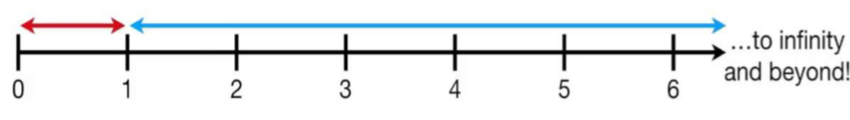
\includegraphics[width=0.4\textwidth]{img/IMG_2212.jpeg}
\end{center}
\begin{equation}
\ln(odds)=\ln(\frac{p}{1-p})=\ln(p)-\ln(1-p)
\end{equation}
\begin{definition}[Logit Transform]
The \textbf{logit} is the natural log of the odds.
\begin{equation}
logit(p)=\ln(odds)=\ln(\frac{p}{1-p})
\end{equation}
\end{definition}
When we compute $\log(odds)$ from pairs of random numbers that add to 100 and plot the results, the histogram forms a normal distribution. This makes $\log(odds)$ valuable for statistics problems involving the probabilities of binary outcomes: win/lose, yes/no, or true/false.
\begin{center}
    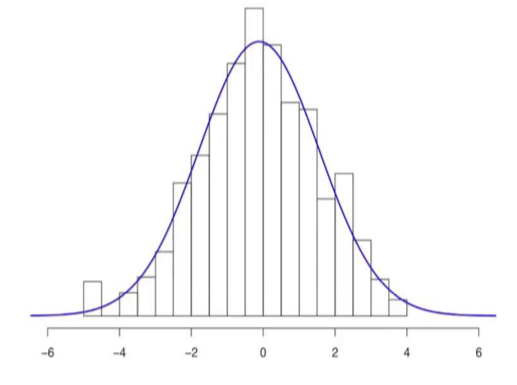
\includegraphics[width=0.3\textwidth]{img/IMG_2214.jpeg}
\end{center}
\begin{table}[h]
\centering
\footnotesize
\begin{tabular}{|c|c|c|}
\hline
\multirow{2}{*}{\textbf{Mutated Gene}} & \multicolumn{2}{c|}{\textbf{Cancer Diagnosis}} \\
\cline{2-3}
& \textbf{Yes} & \textbf{No} \\
\hline
\textbf{Yes} & 23 & 117 \\
\hline
\textbf{No} & 6 & 210 \\
\hline
\end{tabular}
\caption{Contingency table between mutated gene presence and cancer diagnosis}
\label{tab:mutated_gene_cancer}
\end{table}

\begin{example}[(\textbf{Tab \ref{tab:mutated_gene_cancer}}) If someone has the mutated gene, are the odds higher that they will get cancer?]
Working through the numbers, we have:
\[
\frac{\frac{23}{117}}{\frac{6}{210}}=6.88
\]
The odds are 6.88 times greater that someone with the mutated gene will also have cancer.
\begin{equation*}
\log(\text{odds ratio}) = \log(6.88) = 1.93    
\end{equation*}
 

A larger value marks the mutated gene as a strong predictor of cancer, while a smaller one points to a weaker relationship.
\end{example}
\newpage
\begin{table}[h]
\centering
\footnotesize
\begin{tabular}{|c|c|c|c|}
\hline
\multicolumn{1}{|c|}{} & \multicolumn{3}{c|}{\textbf{Sick}} \\
\cline{2-4}
\textbf{Fever} & Yes & No & Total \\
\hline
Normal & 402 & 3614 & 4016 \\
\hline
High & 101 & 345 & 446 \\
\hline
Total & 503 & 3959 & 4462 \\
\hline
\end{tabular}
\caption{Sickness based on fever}
\label{tab:sickness_fever}
\end{table}

\begin{example}[(\textbf{Tab. \ref{tab:sickness_fever}}) The odds of being sick with a Normal value are:]
\begin{align*}
\text{Odds}&(Sick|Normal) &&= \frac{\frac{402}{4016}}{1 - \frac{402}{4016}} = \frac{402}{3614} = 0.111
\\
\text{Odds}&(Not Sick|Normal) &&= \frac{3614}{402} = 8.99
\\
\text{Odds}&(Sick|High) &&= \frac{101}{345} = 0.293
\\
\text{Odds}&(Not Sick|High) &&= \frac{345}{101} = 3.416
\end{align*}
Moving from Normal to High roughly triples the odds of being sick, $\text{Odds ratio} = \frac{0.293}{0.111} = 2.64$: a person is 2.64 times more likely to be sick with a high value.
\end{example}